
\documentclass[journal]{IEEEtran}

\usepackage{amsmath,amssymb,amsfonts}
\usepackage{graphicx}
\usepackage{booktabs}
\usepackage{array}
\usepackage{xcolor}
\usepackage{cite}
\usepackage{textcomp}
\usepackage{algorithm}
\usepackage{algpseudocode}
\usepackage{tikz}
\usetikzlibrary{arrows.meta,positioning,calc,fit,backgrounds,decorations.pathreplacing}

\newcommand{\TBD}[1]{\textcolor{red}{[#1]}}
\newcommand{\NEWRUN}[1]{\textcolor{blue}{[#1]}}
\newcommand{\figph}[3]{%
  \fbox{\parbox[c][#2][c]{\dimexpr#1-2\fboxsep-2\fboxrule\relax}{%
  \centering\footnotesize\textcolor{gray}{\textbf{Figure placeholder}}\\[2pt]
  \parbox{0.9\linewidth}{\centering\footnotesize\textcolor{gray}{#3}}}}}

\begin{document}

\title{An Offline--Online Framework for Real-Time, Constraint-Aware
Predictive Navigation of Magnetic Continuum Robots With a Robot-Mounted
Permanent Magnet}

\author{Anonymous Authors%
\thanks{Manuscript submitted for review to IEEE Transactions on Robotics.}}

\markboth{IEEE Transactions on Robotics}{Offline--Online Predictive
Navigation of Magnetic Continuum Robots}

\maketitle

\begin{abstract}
Steering a magnetic continuum robot (MCR) with a robot-mounted permanent
magnet couples a nonuniform field to the arm's joints and delay, near
the patient. Existing controllers trade model fidelity for speed and rarely enforce
safety inside the optimiser. We present a framework that carries a Cosserat model through to
real-time joint commands with lumen contact modelling.
\end{abstract}

\begin{IEEEkeywords}

\end{IEEEkeywords}

% =============================================================
\section{Introduction}
\label{sec:intro}
% =============================================================

\IEEEPARstart{E}{ndovascular} treatment of stroke and cerebral aneurysm
depends on navigating a guidewire through small, tortuous neurovascular
vessels, often far from the access site. 




This paper presents such a pipeline (Fig.~\ref{fig:framework}). Its
offline layers solve a configuration at every path node, time-parameterise
the path, and precompute a schedule of Jacobians along it. Its online layer
is a delay-aware model predictive controller (MPC) that uses the schedule
to command six joints and insertion, with joint, rate, workspace, and
magnet keep-out constraints enforced inside the quadratic program. The
contributions are:
\begin{enumerate}
\item An offline--online framework that maps joint commands of a
manipulator-mounted permanent magnet to MCR tip motion using a
quasi-static Cosserat model, and runs it in closed loop on hardware with
a 100\,ms control period.
\item An offline Jacobian schedule obtained by implicit differentiation of
the equilibrium, with evidence that a single Jacobian does not generalise
along a path and that the schedule must be computed offline.
\item Delay-aware predictive control with in-QP safety constraints, with
evidence that a controller which checks bounds after the fact is
repeatedly blocked and fails where the MPC tracks along the bound
, and that a longer horizon avoids constraint traps that a
minimal horizon cannot escape.
\item A hardware evaluation on free-space, trap and vessel paths designed
to test one layer each, with a
demonstration of the complete pipeline in a silicone neurovascular model.
% SCOPE 2026-11-11 (rev 2): trap-path claim restored -- planned, scheduled
% later in the campaign, matching framework_main_v2.tex.
\end{enumerate}

% =============================================================
\section{Related Work}
\label{sec:related}
% =============================================================


% =============================================================
\section{Framework Overview}
\label{sec:framework}
% =============================================================

\begin{figure*}[t]
\centering
\figph{\textwidth}{5.0cm}{(a) Platform: UR10e with cylindrical N52
permanent magnet, MCR and insertion advancer, overhead camera,
robot-base frame $\mathcal F_R$, and the 235\,mm magnet keep-out sphere
about the insertion point drawn to scale. (b) Vessel phantom with
centerline and segment C. (c) Rectangle, the three triangles with the height band and keep-out sphere.
(d) MCR cross-section and marker layout. }
\caption{Experimental platform and tasks.}
\label{fig:setup}
\end{figure*}

\begin{figure*}[t]
\centering
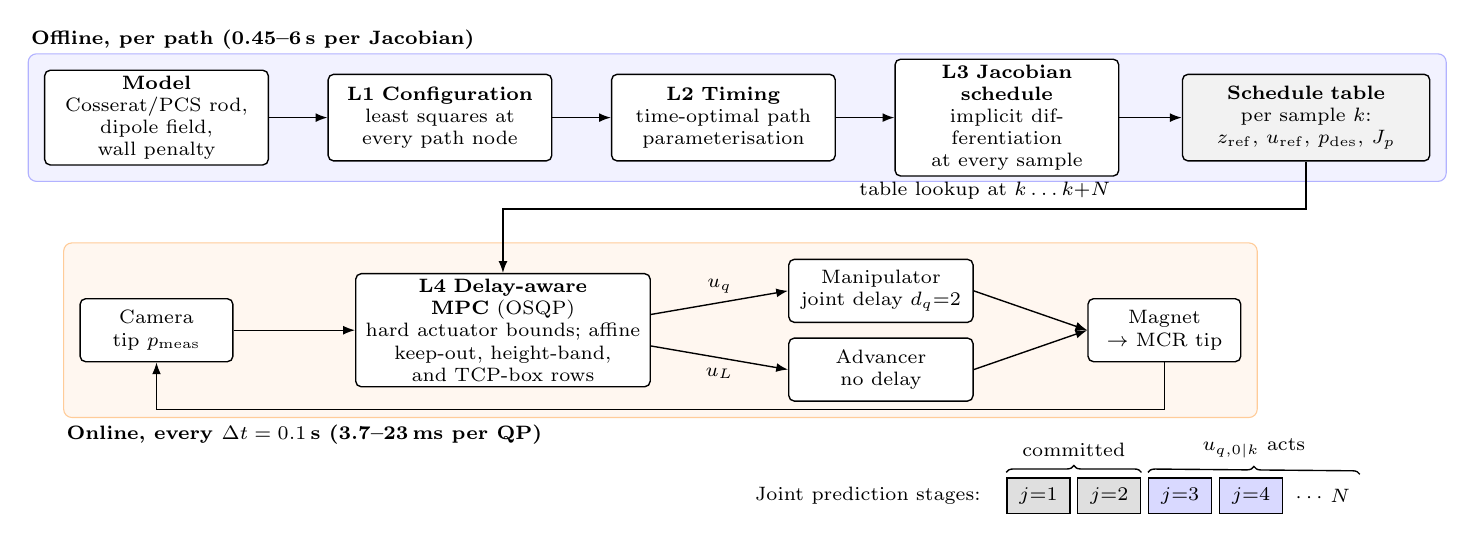
\begin{tikzpicture}[
  font=\scriptsize, >={Latex[length=1.5mm]}, line width=0.5pt,
  lay/.style={draw, rounded corners=2pt, align=center, minimum height=11mm,
              text width=27mm, inner sep=2pt, fill=white},
  on/.style={draw, rounded corners=2pt, align=center, minimum height=8mm,
              inner sep=2pt, fill=white},
  ]
\node[lay] (model) at (0,0) {\textbf{Model}\\Cosserat/PCS rod,\\dipole field, wall penalty};
\node[lay] (l1) at (36mm,0) {\textbf{L1 Configuration}\\least squares at\\every path node};
\node[lay] (l2) at (72mm,0) {\textbf{L2 Timing}\\time-optimal path\\parameterisation};
\node[lay] (l3) at (108mm,0) {\textbf{L3 Jacobian schedule}\\implicit differentiation\\at every sample};
\node[lay, text width=30mm, fill=gray!10] (tab) at (146mm,0) {\textbf{Schedule table}\\per sample $k$:\\$z_{\mathrm{ref}},\,u_{\mathrm{ref}},\,p_{\mathrm{des}},\,J_p$};
\draw[->] (model) -- (l1);
\draw[->] (l1) -- (l2);
\draw[->] (l2) -- (l3);
\draw[->] (l3) -- (tab);
\begin{scope}[on background layer]
\node[fill=blue!5, draw=blue!30, rounded corners=3pt, fit=(model)(tab), inner sep=2mm] (offbg) {};
\end{scope}
\node[anchor=south west, font=\scriptsize\bfseries, inner sep=1pt] at (offbg.north west) {Offline, per path (0.45--6\,s per Jacobian)};
\node[on, text width=18mm] (cam) at (0,-27mm) {Camera\\tip $p_{\mathrm{meas}}$};
\node[on, text width=36mm] (mpc) at (44mm,-27mm) {\textbf{L4 Delay-aware MPC} (OSQP)\\hard actuator bounds; affine\\keep-out, height-band, and TCP-box rows};
\node[on, text width=22mm] (arm) at (92mm,-22mm) {Manipulator\\joint delay $d_q{=}2$};
\node[on, text width=22mm] (adv) at (92mm,-32mm) {Advancer\\no delay};
\node[on, text width=18mm] (mcr) at (128mm,-27mm) {Magnet\\$\rightarrow$ MCR tip};
\draw[->] (cam) -- (mpc);
\draw[->] ([yshift=2mm]mpc.east) -- node[above]{$u_q$} (arm.west);
\draw[->] ([yshift=-2mm]mpc.east) -- node[below]{$u_L$} (adv.west);
\draw[->] (arm.east) -- (mcr.west);
\draw[->] (adv.east) -- (mcr.west);
\draw[->] (mcr.south) -- ++(0,-6mm) -| (cam.south);
\draw[->] (tab.south) -- ++(0,-6mm) -| node[pos=0.2, above]{table lookup at $k\ldots k{+}N$} (mpc.north);
\begin{scope}[on background layer]
\node[fill=orange!6, draw=orange!40, rounded corners=3pt, fit=(cam)(arm)(adv)(mcr), inner sep=2mm] (onbg) {};
\end{scope}
\node[anchor=north west, font=\scriptsize\bfseries, inner sep=1pt] at ([yshift=-0.5mm]onbg.south west) {Online, every $\Delta t=0.1$\,s (3.7--23\,ms per QP)};
\begin{scope}[shift={(112mm,-48mm)}]
\foreach \j/\c in {1/gray!25,2/gray!25,3/blue!15,4/blue!15} {
  \node[draw, minimum width=8mm, minimum height=4.5mm, fill=\c] (s\j) at ({(\j-1)*9mm},0) {$j{=}\j$};
}
\node[anchor=west] (dots) at ($(s4.east)+(0.3mm,0)$) {$\cdots\,N$};
\draw[decorate,decoration={brace,amplitude=2.5pt}] ([yshift=0.6mm]s1.north west) -- node[above=2pt]{committed} ([yshift=0.6mm]s2.north east);
\draw[decorate,decoration={brace,amplitude=2.5pt}] ([yshift=0.6mm]s3.north west) -- node[above=2pt]{$u_{q,0|k}$ acts} ([yshift=0.6mm]dots.north east);
\node[anchor=east, font=\scriptsize] at ([xshift=-2mm]s1.west) {Joint prediction stages:};
\end{scope}
\end{tikzpicture}
\caption{The framework. Offline layers L1--L3 turn a quasi-static model
into a schedule of reference configurations, rates, tip targets and
Jacobians. Online, L4 reads the tip targets and Jacobians over its horizon
and commands six joints
and insertion under actuator bounds and affine geometric constraints; independent monitors re-check the safety bounds from measured joints. Bottom right: because
joint commands act only after $d_q=2$ ticks, the first predicted stage they
influence is $j=3$.}
\label{fig:framework}
\end{figure*}


\subsection{Platform Hardware Configuration}
\label{sec:problem}

A permanently magnetised continuum robot (MCR) is advanced
through a fixed insertion point by a linear advancer. A six-axis
manipulator carries the external permanent magnet that steers the MCR
(Fig.~\ref{fig:setup}, Table~\ref{tab:params}). Unless stated otherwise,
positions are expressed in the robot-base frame $\mathcal F_R$. The
camera measurement is transformed into this frame before it is used by
the controller; \TBD{report the camera-to-robot calibration procedure}.

Let $q\in\mathbb R^6$ denote the manipulator joint angles and $L$ the
inserted length. The manipulator forward kinematics determine the
external magnet position $p_a(q)$ and orientation $R_a(q)$. The vector
$\phi_a(q)\in\mathbb R^3$ denotes the chosen coordinates for that
orientation. The MCR model parameter is
\begin{equation}
\theta(z)=
\begin{bmatrix}
p_a(q)\\ \phi_a(q)\\ L
\end{bmatrix}\in\mathbb R^7,\qquad
z=\begin{bmatrix}q\\L\end{bmatrix}\in\mathbb R^7,
\qquad
u=\dot z,
\label{eq:config}
\end{equation}
where the model insertion length is $\ell=L$. The orientation
coordinates and their derivative map must be consistent with the
manipulator Jacobian used in Section~\ref{sec:l3}. The external magnet
moment in $\mathcal F_R$ is $m_a=R_a(q)m_a^a$, where $m_a^a$ is its
constant moment in the magnet frame.

The controller selects joint and insertion rates $u$ to track a desired
tip-position trajectory while respecting actuator limits and geometric
workspace constraints. The tracking and safety constraints below are
evaluated in the calibrated task frame.

\begin{table}[t]
\centering
\caption{Platform, model, controller, and constraint parameters.}
\label{tab:params}
\footnotesize
\setlength{\tabcolsep}{3.5pt}
\renewcommand{\arraystretch}{1.08}
\begin{tabular}{@{}>{\raggedright\arraybackslash}p{0.45\columnwidth}>{\raggedright\arraybackslash}p{0.51\columnwidth}@{}}
\toprule
\multicolumn{2}{@{}l}{\emph{Platform}} \\
Manipulator & UR10e, External Control URCap \\
Control computer & i7-11700K, 31\,GB RAM \\
Operating system & Ubuntu 22.04, PREEMPT\_RT kernel \\
Manipulator command stream / MPC update & 125\,Hz / 10\,Hz \\
MPC period $\Delta t$ & 0.1\,s \\
Joint / insertion command delay $d_q,d_L$ & 2 / 0 ticks \\
Advancer resolution & 0.166\,mm/step \\
\midrule
\multicolumn{2}{@{}l}{\emph{MCR and magnet model}} \\
MCR diameter / PCS segments $n_s$ & 2.0\,mm / 10 \\
Wire effective modulus $E$ / Poisson ratio $\nu$ & $\approx$2.5\,MPa / 0.49 \\
External magnet & N52 NdFeB cylinder, $100\times100$\,mm \\
Wall stiffness $k_c$ / smoothing length $\varepsilon_c$ &
$10^8$\,N\,m$^{-2}$ / $10^{-5}$\,m \\
\midrule
\multicolumn{2}{@{}l}{\emph{MPC and baseline}} \\
MPC horizon $N$ & 15 (short-horizon ablations: 3 and 1) \\
$Q_p$ / $Q_u$ / $Q_{\Delta u}$ & 1.0 at 0.5\,mm / 7.0 / $10^{-3}$ \\
DLS rate scales $S_u$ (joint / insertion) &
0.05\,rad/s / 5\,mm/s \\
Per-tick rate-increment scales $S_{\Delta u}$ (joint / insertion) &
0.04\,rad/s / 2\,mm/s \\
INV-7 gain $k_p$ / damping $\lambda_u$ &
1.0\,s$^{-1}$ / $2.5\times10^{-3}$\,m/s \\
Error Tracking Threshold & 7 mm\\
\bottomrule
\end{tabular}
\end{table}

$S_u$ is diagonal, with six joint-rate scales and one insertion-rate
scale. $S_{\Delta u}$ gives the per-tick rate-increment scale used to set
$\Delta u_{\min},\Delta u_{\max}$. \TBD{State whether these bounds are
symmetric and give their componentwise values.}


% =============================================================
\begin{table}[tb]
\centering
\caption{Core notation used in the model and controller.}
\label{tab:notation}
\footnotesize
\setlength{\tabcolsep}{3.5pt}
\renewcommand{\arraystretch}{1.08}
\begin{tabular}{@{}>{\raggedright\arraybackslash}p{0.32\columnwidth}>{\raggedright\arraybackslash}p{0.64\columnwidth}@{}}
\toprule
Symbol & Meaning \\
\midrule
$q\in\mathbb R^6$ & Manipulator joint angles \\
$L=\ell$ & Inserted length in the controller / rod model \\
$z$ & $[q^\top,L]^\top$: controlled configuration \\
$u=\dot z$ & Joint and insertion rate command \\
$\theta$ & $[p_a^\top,\phi_a^\top,\ell]^\top$: magnet pose and insertion model input \\
$\xi(s)$ & Rod curvature and twist strain \\
$\mu_r(s)$ & Body-frame MCR moment per unit length \\
$p_{\mathrm{tip}}$, $p_{\mathrm{des}}$ & Modelled tip and desired tip positions \\
$J_p$ & $3\times7$ tip-position Jacobian with respect to $z$ \\
$d_q$, $d_L$ & Joint and insertion command delays, in MPC ticks \\
$N$, $\Delta t$ & MPC horizon and update period \\
\bottomrule
\end{tabular}
\end{table}

\section{Offline Layers: Model, Configuration, Timing, and Jacobians}
\label{sec:offline}
% =============================================================

\subsection{Quasi-Static Magnetic Rod Model}
\label{sec:model}

The MCR is modelled as an inextensible, unshearable Cosserat rod with
piecewise-constant strain (PCS) over $n_s$ segments
\cite{renda2018discrete,edelmann2017magnetic}. Let
$\xi(s)=[\kappa_1(s),\kappa_2(s),\tau(s)]^\top$ denote its two
bending strains and twist, and let $\xi_0(s)$ be the rest strain. With
the local tangent along $e_3$, the rod kinematics and elastic energy are
\begin{equation}
\begin{aligned}
p'(s) &= R(s)e_3,\\
R'(s) &= R(s)\widehat{\xi}(s),\\
W_{\mathrm{el}} &= \frac{1}{2}\int_0^\ell
\bigl(\xi(s)-\xi_0(s)\bigr)^\top\\
&\qquad K\bigl(\xi(s)-\xi_0(s)\bigr)\,ds .
\end{aligned}
\label{eq:rod}
\end{equation}
where $K=\operatorname{diag}(EI,EI,GJ)$, $E$ and $G$ are the Young
and shear moduli, $G=E/[2(1+\nu)]$ for an isotropic wire, and $I$ and
$J$ are the cross-section bending and torsional second moments.
The hat map $\widehat{\cdot}$ converts a vector to its skew-symmetric
matrix. \TBD{Verify that this strain ordering matches the implementation.}

The external magnet is approximated as a point dipole, which is
an appropriate far-field model when the magnet-to-robot distance is
large relative to the magnet dimensions. For a field point $x$, define the displacement from
the external-magnet center as
$\mathbf r=x-p_a$, its magnitude as $r=\|\mathbf r\|$, and its unit
direction as $\widehat{\mathbf r}=\mathbf r/r$. The external magnet's
moment, $m_a$, and $p_a$ are expressed in $\mathcal F_R$.
\begin{align}
B(x;\theta)
&=\frac{\mu_0}{4\pi r^3}
\left[3(\widehat{\mathbf r}^{\top}m_a)\widehat{\mathbf r}-m_a\right],
\label{eq:dipole}\\
W_m
&=-\int_0^\ell
\big(R(s)\mu_r(s)\big)^\top
B\big(p(s);\theta\big)\,ds,
\label{eq:wm}
\end{align}
where $\mu_r(s)$ is the MCR's body-frame magnetic moment per unit
length and $\mu_0$ is the permeability of free space. The sign and
integral form follow from the dipole potential energy
$u_m=-m^\top B$ applied to each rod element~\cite{kim2022magnetic};
thus, $\mu_r$ has units of magnetic dipole moment per unit length
($\mathrm{A\,m}$). This distributed-moment model assumes the MCR's magnetisation
is prescribed and does not change with the applied field.
\TBD{Report measured or identified values of $\mu_r(s)$ and compare the
point-dipole field against a measured field map over the operating
workspace; use a finite-magnet field model if the discrepancy is material.}

In the vessel, contact is represented by the penalty
\begin{equation}
W_c=\frac12 k_c\int_0^\ell
\operatorname{sp}_{\varepsilon_c}(\delta_w(s))^2\,ds,
\label{eq:contact}
\end{equation}
where $\delta_w(s)$ is signed wall penetration (positive inside the
wall) and $\operatorname{sp}_{\varepsilon_c}$ is the smooth positive-part
function. \TBD{Give the exact smoothing function.}
The digitised phantom lumen is used for the vessel-path configuration
solve, Jacobian schedule, and Jacobian validation. Contact energy
vanishes on the free-space paths.

The quasi-static equilibrium is
\begin{equation}
\xi^*(\theta)=\arg\min_\xi\Pi(\xi;\theta),\qquad
\Pi=W_{\mathrm{el}}+W_m+W_c,
\label{eq:equilibrium}
\end{equation}
with the strain bounds used by L-BFGS-B. The solver uses analytic
gradients and is warm-started as insertion increases, following the
equilibrium branch reached by incremental insertion. Inertia is omitted because the model is quasistatic. Gravity does not
appear in $\Pi$ as the phantom lumen model supports the MCR's weight. 

\subsection{L1: Configuration at Every Path Node}
\label{sec:l1}

Let $i=1,\ldots,M$ index path nodes, with $\chi_0$ the
initial/nominal configuration. Let $\chi_i=[q_i^\top,L_i]^\top$
be the configuration at node $i$.
The model insertion length is $\ell_i=L_i$. For desired tip positions
$p_{\mathrm{des},i}$, L1 solves the bounded nonlinear least-squares
problem
\begin{equation}
\begin{aligned}
\chi_i^* &= \arg\min_{\chi_{\min}\leq\chi\leq\chi_{\max}}
\|r_{\mathrm{LS},i}(\chi)\|_2^2,\\
r_{\mathrm{LS},i}(\chi)
&=
\begin{bmatrix}
\big(p_{\mathrm{tip}}(\chi)-p_{\mathrm{des},i}\big)/\sigma_p\\[2pt]
\sqrt{w_r}\,
\big[\|p_a(q)-p_{\mathrm{tip}}(\chi)\|-r_{\max}\big]_+/\sigma_r\\[2pt]
\sqrt{w_c}\,D_c^{-1}(\chi-\chi_{i-1})\\[2pt]
\sqrt{w_0}\,D_0^{-1}(\chi-\chi_0)
\end{bmatrix}.
\end{aligned}
\label{eq:planner}
\end{equation}
Here $p_{\mathrm{tip}}$ is the equilibrium tip position, $p_a(q)$ is
the external-magnet centre, and $[x]_+=\max(0,x)$. The first residual
tracks the path; the second penalizes a magnet-to-tip distance above
$r_{\max}$; the remaining residuals regularize changes from the
previous configuration and departure from nominal posture $\chi_0$.
The matrices $D_c$ and $D_0$ are positive diagonal scale matrices that
normalize the joint-angle and insertion-length components; $w_r,w_c,w_0$
are nonnegative scalar weights. The position scales
$\sigma_p$ and $\sigma_r$ are positive length scales, so all residual
components are dimensionless. \TBD{Give the configuration bounds and
all residual scales and weights. State how the rod equilibrium is
computed during each L1 residual evaluation.}

\subsection{L2: Time Parameterisation}
\label{sec:l2}

The node sequence is assigned timing with reachability-based
time-optimal path parameterisation (TOPP-RA)
\cite{shinmckay1985minimumtime,phampham2018reachability}. A backward
pass computes the controllable set, and a forward pass computes the
fastest feasible speed profile subject to joint and insertion velocity
and acceleration limits. A $C^2$ spline is then fitted and the profile
is dilated to an integer number of MPC periods. The resulting samples are $z_{\mathrm{ref},k}$, the feedforward rate
$u_{\mathrm{ref},k}$, and the desired tip position $p_{\mathrm{des},k}$.
\TBD{Report whether velocity and acceleration limits are rechecked after
spline fitting and time dilation.}

\subsection{L3: Jacobian Schedule by Implicit Differentiation}
\label{sec:l3}

Define $f(\xi,\theta)=\nabla_\xi\Pi(\xi;\theta)$. At an
unconstrained, nondegenerate equilibrium, differentiating
$f(\xi^*(\theta),\theta)=0$ gives
\begin{equation}
H_{\xi\xi}\frac{\partial\xi^*}{\partial\theta}
+H_{\xi\theta}=0,\qquad
\frac{\partial\xi^*}{\partial\theta}
=-H_{\xi\xi}^{-1}H_{\xi\theta},
\label{eq:ift}
\end{equation}
where $H_{\xi\xi}=\partial^2\Pi/\partial\xi^2$ and
$H_{\xi\theta}=\partial^2\Pi/(\partial\xi\,\partial\theta)$.
If strain bounds are active, the derivative must instead be obtained
from the corresponding KKT system. The Hessian blocks are
finite-differenced from the analytic gradient, so no perturbed
equilibrium is re-solved. \TBD{Report finite-difference steps and any
Hessian regularisation.}

Let $h(\xi,\theta)=p_{\mathrm{tip}}$ be the tip-position map. The
base-coordinate sensitivity is
\begin{equation}
J_b=
\frac{\partial h}{\partial\xi}
\frac{\partial\xi^*}{\partial\theta}
+\left.\frac{\partial h}{\partial\theta}\right|_{\xi^*}
\in\mathbb R^{3\times7}.
\label{eq:ift_jac}
\end{equation}
With the manipulator map $\theta=\theta(z)$, the joint/insertion
Jacobian follows by the chain rule:
\begin{equation}
J_p(z)=J_b(\theta(z))\,J_\theta(z),\qquad
J_\theta(z)=\frac{\partial\theta}{\partial z},\qquad
J_p(z)\in\mathbb R^{3\times7}.
\label{eq:joint_jac}
\end{equation}
This chain rule includes the map from joint rates to the chosen
orientation coordinates. \TBD{Specify that coordinate chart and the
orientation-rate conversion used in the implementation.}

The schedule stored with the reference is
\begin{equation}
J_{p,k}=J_p(z_{\mathrm{ref},k}),\qquad k=0,\ldots,K_{\mathrm{ref}}.
\label{eq:schedule}
\end{equation}
The reported wall time per Jacobian is 0.45--0.48\,s on the free-space paths and
0.89--6.0\,s on the vessel paths (Table~\ref{tab:compute}), which is
5--60 times the 0.1\,s MPC period. On vessel paths, the insertion
column is evaluated without the wall term for simplicity.


For conditioning, report $\kappa_2(J_{p,k}S_u)$, where $S_u$ is the
diagonal rate-scale matrix in Table~\ref{tab:params}. Across paths, the
reported range is \TBD{verify: 4.7--208}, with per-path medians of
\TBD{verify: 11.5--23.0}. \TBD{Define how these range and median
statistics are aggregated.}

\begin{table}[t]
\centering
\caption{Computation times on the control computer.}
\label{tab:compute}
\footnotesize
\begin{tabular}{@{}ll@{}}
\toprule
Operation & Wall time \\
\midrule
One free-space Jacobian & 0.45--0.48\,s \\
One vessel-path Jacobian & 0.89--6.0\,s \\
Online QP solve & 3.7--23\,ms \\
\bottomrule
\end{tabular}
\end{table}

\begin{algorithm}[t]
\caption{Offline--online framework}
\label{alg:framework}
\footnotesize
\begin{algorithmic}[1]
\Statex \textbf{Offline, per path}
\For{each path node $i$}
  \State $\chi_i\gets\arg\min\|r_{\mathrm{LS},i}(\chi)\|^2$ from $\chi_{i-1}$ \Comment{L1, \eqref{eq:planner}}
  \State verify $\chi_i$ with the full equilibrium model \Comment{\eqref{eq:equilibrium}}
\EndFor
\State $\{z_{\mathrm{ref},k},u_{\mathrm{ref},k},p_{\mathrm{des},k}\}\gets$ TOPP-RA$(\chi)$ \Comment{L2}
\For{each reference sample $k$}
  \State $J_{p,k}\gets$ implicit derivative at $z_{\mathrm{ref},k}$ \Comment{L3, \eqref{eq:joint_jac}}
\EndFor
\Statex \textbf{Online, every $\Delta t$}
\State read $p_{\mathrm{meas},k}$ and $q_k$; integrate $L_k$; form $b_k$ \Comment{\eqref{eq:offset}}
\State build delayed prediction from $J_{p,k},\ldots,J_{p,k+N}$ \Comment{\eqref{eq:delay}--\eqref{eq:prediction}}
\State linearize the geometric constraints at each stage
\State solve the QP; on deadline miss hold the latest committed setpoint
\State $c_{k+1}\gets c_k+\Delta t\,u_{0|k}$; stream the setpoint
\State independently check bounds from measured joints; stop on violation
\end{algorithmic}
\end{algorithm}

% =============================================================
\section{Online Layer: Delay-Aware Constrained MPC}
\label{sec:online}
% =============================================================

\subsection{Delay-Aware Prediction}
\label{sec:pred}

The controller predicts tip position from the offline schedule. The
manipulator command has a delay of $d_q=2$ MPC ticks; insertion has
$d_L=0$. Let $c_k$ be the latest committed manipulator setpoint and
$c_{k-1}$ the preceding setpoint. Let $u_{q,r|k}$ and $u_{L,r|k}$
denote the joint and insertion components of the rate selected for
future stage $r$. Under this timing convention,
\begin{equation}
q_{j|k}=
\begin{cases}
c_{k-1}, & j=1,\\
c_k, & j=2,\\
c_k+\Delta t\displaystyle\sum_{r=0}^{j-3}u_{q,r|k}, & j\geq3,
\end{cases}
\qquad
L_{j|k}=L_k+\Delta t\sum_{r=0}^{j-1}u_{L,r|k}.
\label{eq:delay}
\end{equation}
Thus stage $j=d_q+1=3$ is the first stage influenced by a newly
selected joint command; insertion responds at the first predicted
stage. Define $z_{j|k}=[q_{j|k}^\top,L_{j|k}]^\top$.

Let $z_{\mathrm{meas},k}=[q_k^\top,L_k]^\top$, where $q_k$ is read
from the manipulator and $L_k$ is integrated from the insertion-rate
command. All tip positions below are expressed in the same task frame.
The measured offset
\begin{equation}
b_k=p_{\mathrm{meas},k}-
\left[p_{\mathrm{des},k}
+J_{p,k}(z_{\mathrm{meas},k}-z_{\mathrm{ref},k})\right]
\label{eq:offset}
\end{equation}
corrects the local affine model at the current measurement. It is held
constant over the prediction horizon. With
$\delta z_{j|k}=z_{j|k}-z_{\mathrm{ref},k+j}$, the predicted tip
position is
\begin{equation}
\hat p_{j|k}
=p_{\mathrm{des},k+j}
+J_{p,k+j}\delta z_{j|k}+b_k.
\label{eq:prediction}
\end{equation}
Each stage uses its own scheduled Jacobian. The frozen-Jacobian (FJ)
ablation replaces all $J_{p,k+j}$ by the trial-start Jacobian. For
vessel paths this is evaluated at the measured start configuration;
the relative difference from the planned initial Jacobian is reported
as approximately $10^{-4}$. \TBD{Define the relative-difference norm
in the Results section.}

\subsection{Constrained Quadratic Program}
\label{sec:mpc}

The MPC decision vector is
$U=[u_{0|k}^\top,\ldots,u_{N-1|k}^\top]^\top$. Define
$u_{-1|k}=u_{k-1}$ as the previously applied rate and
$\Delta u_{j|k}=u_{j|k}-u_{j-1|k}$. With
$\|x\|_W^2=x^\top W x$, the QP is
\begin{equation}
\begin{aligned}
\min_U\quad&
\sum_{j=1}^{N}
\|\hat p_{j|k}-p_{\mathrm{des},k+j}\|_{Q_p}^2\\
&+\sum_{j=0}^{N-1}
\left(
\|u_{j|k}-u_{\mathrm{ref},k+j}\|_{Q_u}^2
+\|\Delta u_{j|k}\|_{Q_{\Delta u}}^2
\right)\\
\text{subject to}\quad&
u_{\min}\leq u_{j|k}\leq u_{\max},\quad j=0,\ldots,N-1,\\
&\Delta u_{\min}\leq\Delta u_{j|k}\leq\Delta u_{\max},\quad j=0,\ldots,N-1,\\
&z_{\min}\leq z_{j|k}\leq z_{\max},\quad j=1,\ldots,N,\\
&g_{\mathrm{lin},j}(z_{j|k})\leq0,
\qquad j=1,\ldots,N .
\end{aligned}
\label{eq:mpc}
\end{equation}
Here $Q_p\in\mathbb R^{3\times3}$ and
$Q_u,Q_{\Delta u}\in\mathbb R^{7\times7}$ are positive semidefinite
weighting matrices. \TBD{Give their numerical matrices or exact
normalised diagonal entries.} The feedforward term
$u_{\mathrm{ref}}$ pulls the total commanded rate toward the planned
rate, while the tracking term can move it away from the plan.

The rows $g_{\mathrm{lin},j}$ are affine approximations of the
magnet-centre keep-out sphere (235\,mm radius about the insertion
point), the magnet height band, and the TCP box. \TBD{Give each exact
nonlinear constraint, linearization point, and robust margin.}
The QP constraints act on queued setpoints and account for the two-tick arm
delay using \eqref{eq:delay}. These affine constraints define
feasibility for the QP model; the nonlinear constraints are also
recomputed from measured joints by an independent monitor.

The QP is solved by OSQP~\cite{osqp2020}; only $u_{0|k}$ is applied.
The setpoint accumulator is seeded at the measured start configuration
and updated as
\begin{equation}
c_{k+1}=c_k+\Delta t\,u_{0|k}.
\label{eq:accumulator}
\end{equation}
The MPC updates every 0.1\,s (10\,Hz), while a separate thread streams
the latest committed setpoint to the manipulator interface at 125\,Hz.
On a missed MPC deadline, the latest committed setpoint is held.
The independent monitor recomputes magnet distance and height from
measured joints and checks the TCP in its monitoring frame; any
violation stops the trial. A trial also stops when the measured
tracking error exceeds the threshold in Table~\ref{tab:params}.


\subsection{Baseline: Matched-Authority Inverse-Jacobian Control}
\label{sec:inv7}

The baseline uses the same scheduled Jacobian, delay model, rate scales,
and actuator limits as the MPC, but checks geometric constraints after
computing a correction. Let $i_k$ be the current reference index.
The first reference sample affected by a new joint command is at
relative stage $j_\kappa=1+d_q$ and absolute index
$\kappa_k=i_k+j_\kappa$.
Define $e_{\kappa_k}=p_{\mathrm{des},\kappa_k}-\hat p^{\mathrm{hold}}_{j_\kappa|k}$,
where $\hat p^{\mathrm{hold}}$ is evaluated with no newly selected
joint correction using \eqref{eq:offset}--\eqref{eq:prediction}. Define
$J_{u,\kappa}=J_{p,\kappa}S_u$, where $S_u$ is the diagonal matrix of
rate scales. One damped least-squares rate command is
\begin{equation}
u^{\mathrm{INV}}_k
=S_uJ_{u,\kappa_k}^\top
\left(J_{u,\kappa_k}J_{u,\kappa_k}^\top
+\lambda_u^2I\right)^{-1}
k_p e_{\kappa_k}.
\label{eq:inv7}
\end{equation}
This is the scaled damped least-squares inverse
\cite{wampler1986dls}. The gain $k_p$ has units of inverse seconds,
and $\lambda_u$ is expressed in task-velocity units after rate
scaling. Rate and per-tick rate-increment limits are applied by
clipping. The geometric constraints are not included in the
correction: if the candidate setpoint violates a bound, that command
is blocked and the manipulator holds its previous setpoint for that
tick.

The gain $k_p=1.0\,\mathrm{s}^{-1}$ was selected to place INV in the
same rate-saturation regime as the MPC. The predecessor controller
saturated on 20.5\% of ticks at this gain. \TBD{Report the saturation
fraction for each controller on the current paths and identify the
condition associated with the $0.6$ gain in Table~\ref{tab:params}.}

\begin{thebibliography}{99}
\footnotesize


\bibitem{renda2018discrete}
F.~Renda, F.~Boyer, J.~Dias, and L.~Seneviratne, ``Discrete Cosserat
approach for multisection soft manipulator dynamics,'' \emph{IEEE Trans.
Robot.}, vol.~34, no.~6, pp.~1518--1533, Dec. 2018.


\bibitem{byrd1995lbfgsb}
R.~H. Byrd, P.~Lu, J.~Nocedal, and C.~Zhu, ``A limited memory algorithm
for bound constrained optimization,'' \emph{SIAM J. Sci. Comput.},
vol.~16, no.~5, pp.~1190--1208, 1995.


\bibitem{shinmckay1985minimumtime}
K.~G. Shin and N.~D. McKay, ``Minimum-time control of robotic
manipulators with geometric path constraints,'' \emph{IEEE Trans. Autom.
Control}, vol.~30, no.~6, pp.~531--541, Jun. 1985.

\bibitem{phampham2018reachability}
H.~Pham and Q.-C. Pham, ``A new approach to time-optimal path
parameterization based on reachability analysis,'' \emph{IEEE Trans.
Robot.}, vol.~34, no.~3, pp.~645--659, Jun. 2018.
\bibitem{osqp2020}
B.~Stellato, G.~Banjac, P.~Goulart, A.~Bemporad, and S.~Boyd, ``OSQP: An
operator splitting solver for quadratic programs,'' \emph{Math. Program.
Comput.}, vol.~12, no.~4, pp.~637--672, 2020.



\bibitem{wampler1986dls}
C.~W. Wampler II, \textquotedblleft Manipulator inverse kinematic
solutions based on vector formulations and damped least-squares
methods,\textquotedblright{} \emph{IEEE Trans. Syst., Man, Cybern.},
vol.~16, no.~1, pp.~93--101, 1986.

\bibitem{edelmann2017magnetic}
J.~Edelmann, A.~J. Petruska, and B.~J. Nelson, ``Magnetic control of
continuum devices,'' \emph{Int. J. Robot. Res.}, vol.~36, no.~1,
pp.~68--85, 2017, doi: 10.1177/0278364916683443.


\bibitem{kim2022magnetic}
Y.~Kim and X.~Zhao, ``Magnetic soft materials and robots,''
\emph{Chem. Rev.}, vol.~122, no.~5, pp.~5317--5364, 2022,
doi: 10.1021/acs.chemrev.1c00481.

\end{thebibliography}

\end{document}
